\documentclass[conference]{IEEEtran}
\IEEEoverridecommandlockouts
% The preceding line is only needed to identify funding in the first footnote. If that is unneeded, please comment it out.
\usepackage{cite}
\usepackage{amsmath,amssymb,amsfonts}
\usepackage{algorithmic}
\usepackage{graphicx}
\usepackage{textcomp}
\usepackage{xcolor}
\def\BibTeX{{\rm B\kern-.05em{\sc i\kern-.025em b}\kern-.08em
    T\kern-.1667em\lower.7ex\hbox{E}\kern-.125emX}}
\begin{document}

\title{Hardware-aware Neural Architecture Search\\}

\author{\IEEEauthorblockN{Annika {\"O}sterdiekhoff}
\IEEEauthorblockA{\textit{Embedded Systems Research Group} \\
\textit{University of Duisburg-Essen}\\
Duisburg, Germany \\
annika.oesterdiekhoff@stud.uni-due.de}
}

\maketitle

\begin{abstract}
Neural Architecture Search is a grown topic for automatic design of deep learning models. With the rise of IoT and mobile devices nowadays in combination to the raising popularity of deep learning models, researchers try to fit deep learning models on specific hardware. Using different hardware can lead to restrictions in memory size, latency and computational power. Therefore, hardware-aware NAS is developed which does not only consider to maximize the accuracy of a deep learning model but also the usability on a specific hardware platform measured by FLOPs, model size, latency, energy consumption, etc. This paper gives a brief overview about hardware-aware neural architecture search by focusing on model optimization techniques, the problem definition of hardware-aware NAS, its search space and search strategy and its challenges and limitations.  
\end{abstract}

\begin{IEEEkeywords}
Hardware-aware Neural Architecture Search, Optimization, Quantization, Hardware Platforms
\end{IEEEkeywords}

\section{Introduction}
\label{section:Introduction}
Deep learning models are gaining more and more interest in various subjects for example in image recognition \cite{bib2} or Natural Language Processing \cite{bib3}. These deep learning models consist of different layers and parameters. Layers are operators like convolution or activation whereas parameters also known as hyper-parameters are pre-defined properties of the architecture or the training algorithm. Architecture parameters are for example the stride and filter size of a convolution layer whereas a training parameter can be the number of epochs. In contrast to these hyper-parameters there exist parameters which are trained in the training process and thus are not fixed at the beginning of the training. Examples of these parameters are the weights of each layer or the bias. 

There are lots of possibilities to build up a deep learning model out of layers and parameters. So, it is difficult for the developer to design the number and type of nodes and the connection between them because of the multiple differences in data types, tasks and hardware platforms. Therefore, most of the deep learning models are created by hand with multiple experiments or are a variation of already known models which work well. This process of creating and designing a model is very time-consuming and costly, therefore techniques are created in the last years to automate the designing process of a deep learning model. One of them is called Neural Architecture Search (NAS). The focus of this paper is a subgroup of NAS, the hardware- or platform-aware NAS (HW-NAS). The goal of HW-NAS is to use NAS for designing a deep learning model but with respect to optimize the deep learning model for a specific hardware device. Possible target hardware platforms can be server processors like CPUs, GPUs, FPGAs and ASICs, mobile devices or tiny devices. For giving an overview about hardware-aware NAS we summarize a recent survey from 2021 \cite{bib1}. 

In the following we define a general NAS process in Section \ref{section:NASDefinition}. In Section \ref{section:ModelOptimization} possible ways to optimize a deep learning model are listed. We distinguish between single-objective and multi-objective optimization in Section \ref{section:ProblemFormulation}. After explaining the architecture and hardware search space in Section \ref{section:SearchSpaces}, the goals of hardware-aware NAS are defined in Section \ref{section:Goals}. We go into detail with the accuracy evaluation method, the hardware cost evaluation method and the search algorithms in Section \ref{section:SearchStrategy}. The NAS frameworks and especially the Microsoft NNI Framework are shortly presented in Section \ref{section:Frameworks}. In the end we define the challenges and limitations in Section \ref{section:Challenges} by speaking about reproducibility, transferability across different hardware platforms and the carbon footprint.  

\section{Neural Architecture Search Definition}
\label{section:NASDefinition}
A neural architecture process firstly includes a \textbf{search space} which consists of possible operators and its connections which create an architecture. The \textbf{search strategy} explores this search space and searches for possible architecture candidates. Then the \textbf{evaluation methodology} is used to train the models and evaluate the accuracy of each model. The models with a high accuracy help to redefine the search space. The whole NAS process is shown in Figure \ref{fig:NASProcess} \cite{bib1}. This search space with multiple architectures and the training of all models cause time consumption and large memory footprints. This leads to a lack of using NAS for constrained hardware or in real-time. Therefore, more and more research is focused on solving this issue by developing hardware-aware NAS. 

\begin{figure}[htbp]
\centerline{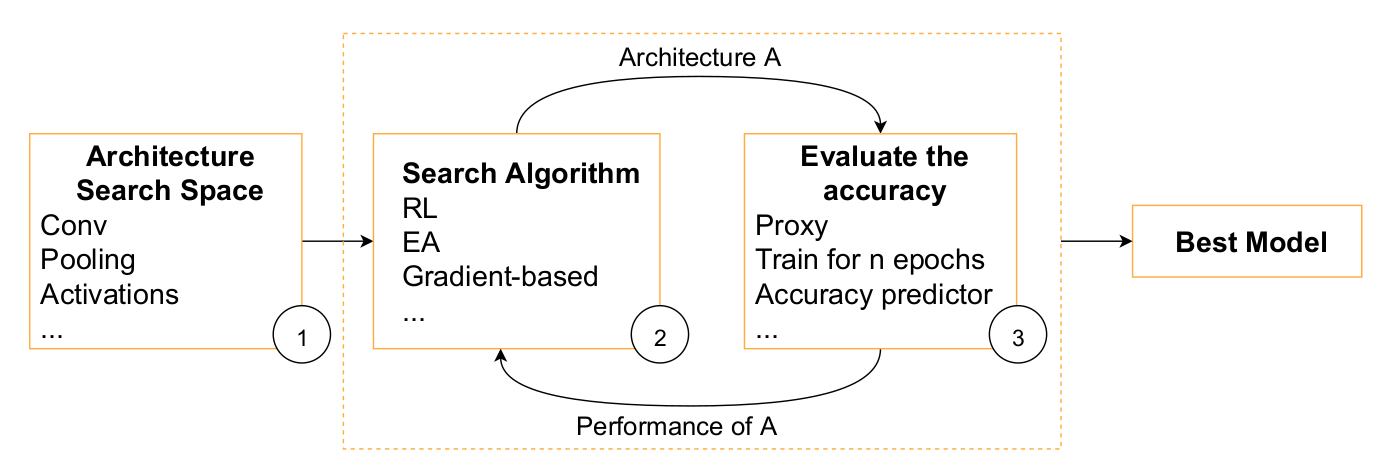
\includegraphics[width=\linewidth]{NASProcess.png}}
\caption{NAS Process\cite{bib1}}
\label{fig:NASProcess}
\end{figure}

\section{Model Optimizations}
\label{section:ModelOptimization}
For solving the drawbacks mentioned above of getting large deep learning models and long training processes, there are some techniques to optimize it.

Firstly one can \textbf{compress a model} by decreasing the model size but gaining the same accuracy. Compressing a model can be done for example by \textit{compacting the model} which changes the standard operations to more simpler operations. In addition, one can \textit{decompose the tensor} which means we shrink the tensors which reduces the size of the deep learning model. What we will mainly focus on for compressing a model is \textit{quantization}. Quantizations means that we convert floating point weights and activation's into smaller digits, ideally binaries. This change of representation can be different in each layer, this is called mixed-precision quantization. Another option for compressing a model is \textit{pruning} where the least important weights or operations are pruned to reduce the model size. The importance of a weight or operation can be the weight itself or has to be learned. There is put lots of effort the last years to automate mixed-precision quantization as well as the pruning. 

In addition one can apply \textbf{hardware-aware NAS} which uses model compressions and takes the usability on a specific hardware platform into account by searching the model from a set of architectures. A relatively new technique for optimizing a deep learning model is \textbf{code transformation} which optimizes the operators of a model for a specific hardware.

Figure \ref{fig:Optimization} \cite{bib1} shows the input and output of compressing a model or applying hardware-aware NAS for optimizing a model. HW-NAS uses intern a model compression method, this means model compression is a subgroup inside HW-NAS.

\begin{figure}[htbp]
\centerline{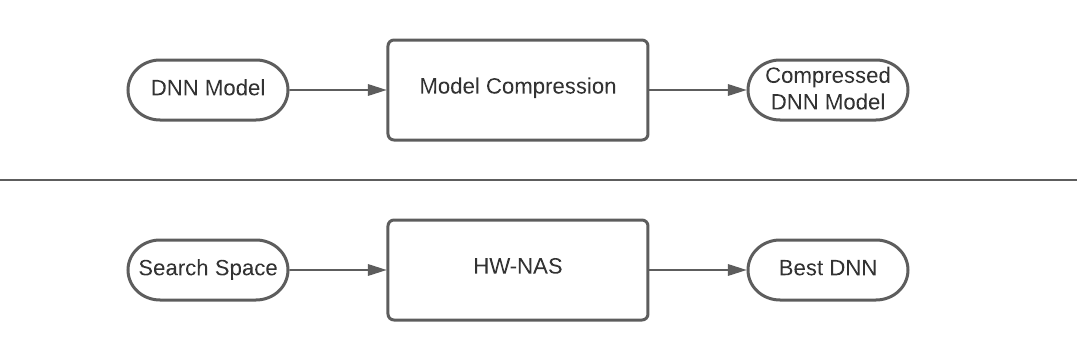
\includegraphics[width=\linewidth]{Optimization.png}}
\caption{Process of optimizing a model by model compression or HW-NAS \cite{bib1}}
\label{fig:Optimization}
\end{figure}

\section{Hardware-Aware NAS Problem Formulation}
\label{section:ProblemFormulation}
In the following we discuss the problem formulation of hardware-aware NAS. In general, NAS is an optimization problem which searches for an architecture which maximizes some specific performance metrics. The performance metric is usually the accuracy. The formula is shown in ``\eqref{eqn:single-obj}''. 
 
\begin{equation}
\label{eqn:single-obj}
\max_{\alpha\epsilon A}\,f(\alpha, \delta)
\end{equation}

So, $A$ is the search space which includes the set of architectures and $\alpha$ is one architecture from this set. $\delta$ is the used data set and $f$ is the performance measure, i.e. the accuracy. The formula says that we try to find the architecture $\alpha$ of the search space $A$ which maximizes the accuracy $f$ for the used data set $\delta$. 
 
By doing hardware-aware NAS one has not only the accuracy metric which should be maximized but also hardware objectives like for example latency. There exist two different problem formulation for hardware-aware NAS, the single and multi-objective optimization.

\subsection{Single-Objective Optimization}

Single-objective optimization means that only one objective is maximized like explained above for example the accuracy. For solving the problem of also having hardware objectives one tries to transform the multi-objective optimization into a single-objective optimization. For doing this there exist two methods. \textbf{Two-Stage optimization} means that we use the problem formulation of original NAS which maximizes the accuracy and optimize in the second stage the architecture for a specific target. This method often does not work well because the best found architecture in the first stage is maybe not the best for the specific target hardware. The alternative to this method is \textbf{constrained optimization}. Here we again try to find the architecture with the highest accuracy but we define some thresholds for hardware constrains like latency or energy consumption which are not allowed to be exceeded by the found architecture. 

\subsection{Multi-Objective Optimization}

The difference to the single-objective optimization which is used in original NAS is multi-objective optimization. The formula is shown here: ``\eqref{eqn:multi-obj}''.
 
\begin{equation}
\label{eqn:multi-obj}
\max_{\alpha\epsilon A}\,f_{1}(\alpha, \delta),f_{2}(\alpha, \delta),\ldots ,f_{n}(\alpha, \delta)
\end{equation}     

Again, $A$ is the search space, $\alpha$ is one of the architectures from the search space and $\delta$ is the used data set. The $f_{1}, f_{2}, ..., f_{n}$ are the performance measures, for example again accuracy but also latency or memory size. Hence, we try to find the architecture $\alpha$ of the search space $A$ which maximizes all performance measures $f$. 

So we now do not only have the accuracy which we have to optimize but various objectives, e.g. latency and energy consumption. These objectives can be conflicting each other for example try to have a minimal search space and gaining the best accuracy. When this occurs we can only try to find the Pareto-optimal solution. The Pareto-optimal solution is a set of architectures where the changing of one measurement, for example improving the accuracy, always leads to a decrease for a different measurement, for example higher latency. It is not possible to improve one objective without drawbacks to the other objectives.

There exist two approaches for this. Firstly the \textbf{scalarization method} which includes the performance measurements $f$'s into one aggregation function like a weighted sum or weighted product. This transforms the multi-objective optimization into a single-objective optimization. Unfortunately by having fixed weights in the aggregation function, it could be that not all Pareto solutions are found. For solving this issue one can run multiple runs which on the other hand then again leads to more needed computing power etc. Another method to find the Pareto-optimal solution is defining \textbf{heuristics}. By doing this one does not form the multi-objective optimization problem into a single-objective one and therefore get a set of architectures as solutions along the Pareto front. An example is the evolutionary NSGA-II algorithm \cite{bib14} which divides the architectures into fronts by means of their dominance. For all architectures is the crowding distance calculated which is the sum of all neighborhood distances across all objectives. This crowding distance is used as priority for the architectures.  

The Figure \ref{fig:ProblemFormulation} is leaned on a figure of the survey \cite{bib1} we summarize and shows the different possibilities of formulating the NAS problem.

\begin{figure*}[htbp]
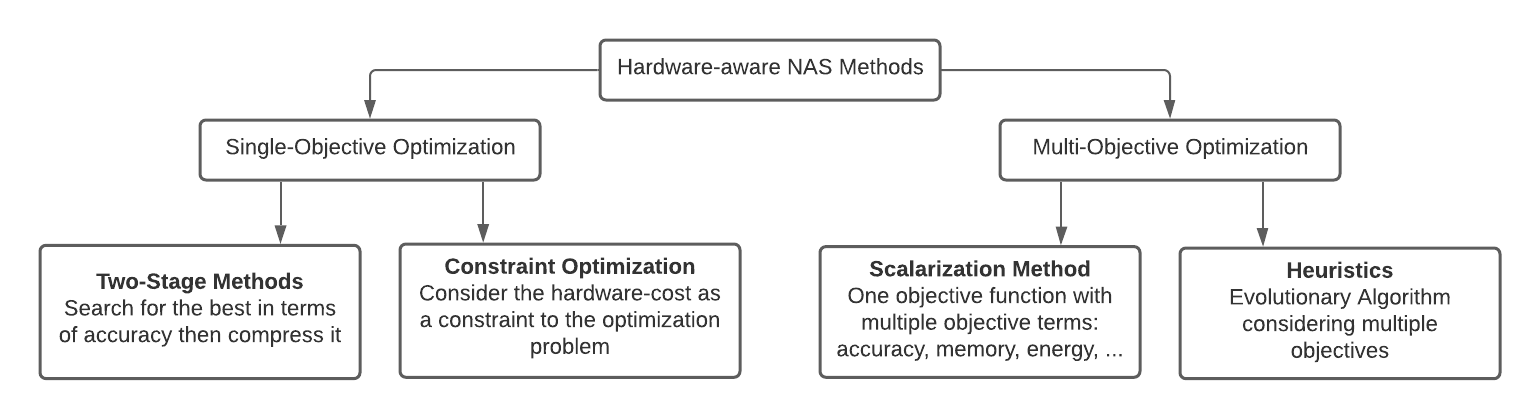
\includegraphics[width=\textwidth]{ProblemFormulation.png}
\caption{Problem formulation of the NAS process \cite{bib1}}
\label{fig:ProblemFormulation}
\end{figure*} 

\section{Search Spaces}
\label{section:SearchSpaces}
There exist two search spaces used by the search strategies of hardware-aware NAS. 

\subsection{Architecture Search Space}
The first one is the Architecture Search Space. It defines a set of architectures which means a set of possible operators and their connections. For designing an architecture search space one can use one \textbf{fixed architecture} and only search for the best architecture hyper-parameters. Unfortunately this needs some knowledge of the human which designs the architecture, but it reduces the size of the search space. On the other hand one can do a search without a fixed architecture and search for \textbf{fitting operators and their connections} of a set of operators and connections. This does not need knowledge of the human how the architecture structure should look like but of course it produces a bigger search space size and with this also a longer search time. By searching for the best architecture without a fixed architecture one distinguishes between three types. Firstly one can have a \textit{layer-wise search space} where the architecture is searched out of a set of operators. Another option is to use a \textit{cell-based search space}. A cell is defined as a graph that includes some operators. A cell-based search space creates an architecture by repeating a found cell multiple times. This mostly leads to a high accuracy but it limits the flexibility in hardware specialization by stacking the same cells. In addition, there exist the \textit{hierarchical search space}. The architecture is build by constructing blocks out of a defined number of different cells. This solves the missing flexibility of the cell-based search space because one does not only stack the same cells on top of each other. 

In the past most NAS researchers defined the type of a network which should be found by the algorithm. Possible types are for example convolutional neural networks (CNNs) or recurrent neural networks (RNNs). The trend now switches to not restrict the search too much in one network type. 

\subsection{Hardware Search Space}
The second possible search space is the Hardware Search Space. This means before evaluating the architectures one already does some hardware optimizations like tuning the tiling parameters. Unfortunately, it is not possible to add all hardware specifications in the search space for optimizing because it would explode the search space and in combination the search space time. So, beforehand hardware optimizations cannot consider all hardware specifications.

In general, there exist two different types of hardware search space. The search space can be \textbf{parameter-based} which means that the search space is a set of optimizing parameters, e.g. tiling parameters or buffer sizes. On the other hand a search space can be \textbf{template-based}. So the search space consists of a set of pre-configured templates instead of optimizing parameters. The idea is to use already known successful designs as templates.

\section{Goals of hardware-aware NAS}
\label{section:Goals}
There are three categories of goals of hardware-aware NAS. Firstly, the category \textbf{single target, fixed configurations} where most hardware-aware NAS belongs to. Single target means that the NAS tries to find the best architecture for one single hardware target. Fixed platform configuration means that we do not change the hardware configuration like for example tiling parameters. The hardware platform configuration is fixed beforehand. We divide this category further in hardware-aware search strategy and hardware-aware search space. The \textit{hardware-aware search strategy} focuses on solving the NAS as a multi-objective problem which means that the accuracy is taken into account as always but also some hardware measurements for example latency. The opposite to this is the \textit{hardware-aware search space} where the NAS works with only a pool of architectures. The bad working architectures on the target hardware are eliminated. It helps to have a prior knowledge for the target platform for creating the set of architectures. The NAS considers then only the accuracy for this set of architectures and no hardware measurements.

The second category of goals of hardware-aware NAS is \textbf{single target, multiple configurations}. This category is very similar to the hardware-aware search space of the above category but it extends the approach. We now have multiple platform configurations and add to the architecture search space the hardware search space. The hardware search spaces tries to find the best hardware architecture for the target hardware configurations by testing for example different tiling configurations. On the other side the architecture search space tries to find the best architecture of the deep learning model. So together, the goal is to find the best architecture in terms of the best platform configuration in combination with the accuracy. 

In addition, there is the category \textbf{multiple targets}. This means one does not focus on one specific hardware like FPGAs but searches for the best architecture for multiple hardware platforms. This approach is the most desirable one because it allows one to port the best architecture to different hardware platforms. But it is also the most challenging one because architectures perform differently on different hardware. We also consider this problem for having an architecture for multiple platforms in Section \ref{section:Challenges}. 

\section{Search Strategies}
\label{section:SearchStrategy}

The search strategy of hardware-aware NAS consists of three elements: an accuracy evaluation method, a hardware cost evaluation method and a search algorithm. 

\subsection{Accuracy Evaluation Method}
The accuracy is evaluated by training the architectures of the search space and comparing the accuracies. Because it would be very time and computational consuming to train all architectures completely, there exist some methods for estimating the accuracy without a training. First, one can \textbf{share weights} between different models to reduce the search time. Second method for speeding up the determination of the accuracy is \textbf{early stopping}. This means one train a deep learning model only a few epochs and uses the accuracy as an approximation for a complete training. In addition, one can include \textbf{hot start}. Hot starting an architecture search means that the searching and training of an architecture is not started with a random model but with an already known efficient model. Furthermore, \textbf{proxy data set} can be used to train the deep learning model with just some data elements and only increase the number in the last steps. In the end there also exist already some \textbf{accuracy prediction models} which use the architecture and data set for predicting the accuracy beforehand. 

\subsection{Hardware Cost Evaluation Method}
Hardware cost evaluation methods are methods for measuring hardware metrics in real-time or as an estimation. A possible hardware measurement are the \textbf{FLOPs and Model Size}. FLOPs are floating point operations. This means the number of floating point operations and the number of parameters as the model size are used as hardware cost measurement. Unfortunately, the number of FLOPs do not completely correlate with the execution time. Thus, FLOPs are not a good indicator to search for efficient architectures, but a small model size leads to fewer memory consumption and automatically searches for compressed models. So, the combination of FLOPs and the model size can be used as a hardware measurement. Another option is to measure the \textbf{latency}. A low latency is important for using NAS in real world applications for ensuring a fast action. Also, the \textbf{energy consumption} measurement can be used as metric for hardware cost evaluation. Possibilities are to use the peak of an energy consumption or the average consumption. Furthermore, the \textbf{area} is considered which means that it is taken into account to gain the smallest possible chip by evaluating the hardware cost. The area also correlates with the power consumption as well. In the end the \textbf{memory footprint} can be considered as a hardware measurement. As said above the number of parameters from a model is a good indicator for measuring the memory footprint. Another better option is to measure the memory consumption while running. 

\subsection{Calculation of FLOPs and Model Size}
In our future work we will use the FLOPs and model size as the numbers of parameters as our hardware cost measurement. Therefore, we present the calculation of FLOPs for a convolutional layer and a fully connected layers which are the layers we will use in our future work very likely \cite{bib5}. The calculation of FLOPs for a convolutional layer is shown in equation ``\eqref{eqn:FLOPs}''.

\begin{equation}
\label{eqn:FLOPs}
FLOPs = 2HW(C_{in}K^{2}+1)C_{out}
\end{equation} 

In the formula equation ``\eqref{eqn:FLOPs}'' stands $H$ for the height of the input, $W$ for the width of the input, $C_{in}$ are the number of input channels, $K$ is the kernel width and $C_{out}$ is the number of output channels. We assume a symmetric kernel width. 

The calculation of FLOPs for the fully connected layer is presented in ``\eqref{eqn:FLOPsFCL}'' whereby $I$ is input dimensionality and $O$ is output dimensionality. 

\begin{equation}
\label{eqn:FLOPsFCL}
FLOPs = 2(I-1)O
\end{equation} 

On the other side the calculation of the model parameters for convolutional layers is done as follows \cite{bib6}:

\begin{equation}
\label{eqn:Params}
Params = C_{in}K^{2}C_{out}+C_{out}
\end{equation} 

Again, the $K$ is the kernel width which is assumed symmetric. $C_{in}$ is the number of input channels as well as $C_{out}$ the number of output channels. When there is no bias, the formula ``\eqref{eqn:Params}'' is reduced to $Params = C_{in}K^{2}C_{out}$. 

The formula of calculating the number of parameters for a fully connected layer is shown in ``\eqref{eqn:ParamsFCL}'' whereby again $I$ is the input dimensionality and $O$ is the output dimensionality. 

\begin{equation}
\label{eqn:ParamsFCL}
Params = IO+O
\end{equation}  


\subsubsection{Real World Measurements versus Estimation models}

Of course real world measurements are very good for evaluating the hardware cost because we are getting a very precise accuracy. But real world measurements have some drawbacks. Mostly, it is very costly. One has to have all used hardware platforms available. In addition, the searching for the best architecture runs longer when trying to get more precise accuracy. Therefore, there exist estimation models like prediction models, lookup tables or a computation of an analytical estimation. In general, prediction models speed up the search time the most. After this follow the lookup tables and then the analytical estimation. But the problem of creating some of these estimation models is that the developer needs hardware experiences and knowledge for making an estimation about the hardware cost. Hence by doing hardware-aware NAS one has to evaluate for each use-case if real world measurements or estimation models work better for calculating the hardware cost. 

\subsection{Search Algorithm}
The search algorithm samples the architectures from the search space and updates the search space for getting architectures with a higher accuracy.
The two most used search algorithms in NAS are reinforcement learning and evolutionary algorithms. By using \textbf{reinforcement learning} an agent chooses between actions in an environment and gets an reward after each action. Its goal is to maximizes the reward so the decision of next actions are based on this. By using reinforcement learning for hardware-aware NAS one action is the sampling of one architecture and the reward is the accuracy and the hardware cost. Therefore, the sampling depends on gaining a high accuracy and low hardware costs. In contrast to this are the \textbf{evolutionary algorithms}. They have three main characteristics: population-based, fitness-oriented and generations. So in the first step the population-based characteristic is applied, which means that the algorithm starts with a set of candidate architectures which are known as population. Then fitness-oriented means that each solution of the set has a quality which is express with its fitness score. For improving this fitness score for different architectures, the evolutionary algorithms can make mutations and crossover operations for generating a new generation/population. The best architectures are used as the new starting point for making new generations of populations and calculate again the fitness score. 

Other possible search algorithms are for example \textbf{gradient-based methods}. Instead of separating the search and the evaluation which is time and computational consuming, one creates a super-network which can simulate any child model. So parts of the model can share their weights which reduces the search time. By training the super-network one gets the weights and parameters for all child architectures. Another option is \textbf{random search} which is the easiest way by just randomly search an architecture but it consumes a lot of time in searching. 

\section{NAS Frameworks}
\label{section:Frameworks}

There are multiple frameworks for applying NAS, for example Auto-Keras, Google AutoML, IBM NeuNets, TPOT, Microsoft Archai, deci.ai AutoNAC, Darwin and Microsoft NNI. All these frameworks have their advantages and disadvantages and focus on different use-cases. We focus on the \textbf{Microsoft Neural Network Intelligence (NNI)} framework because it seems to fit the best for our future work. Microsoft NNI can be used to better compare, reproduce and experiment with various NAS algorithms. It helps the researcher to design their neural network architecture for example by helping with the definition of a super network. It concentrates on the efficiency of the automation by doing NAS. In addition, researcher can use existing NAS algorithms and can easily modify them. Except for AutoNAC, all existing frameworks are not hardware-aware, but Google AutoML and Microsoft NNI support compression methods for specializing the target platform. 

\section{Challenges and Limitations}
\label{section:Challenges}

In the following we list various challenges and limitations of hardware-aware NAS. 

\subsection{Reproducibility}

For providing comparison, it should be possible to reproduce a NAS process. But this is difficult because of the huge possibilities of search spaces, training methods, computational resources and especially for hardware-aware NAS possibilities of hardware devices. There already exist some benchmarks for providing reproducibility but there is a need for more benchmarks to validate own results.
 
\subsection{Transferability of the hardware-aware NAS across multiple Platforms}

One interesting topic in hardware-aware NAS is to design an architecture and transfer it to multiple different platforms. The problem hereby is the variety and different complexities of the hardware platforms. For solving this issue there exist two approaches.

\subsubsection{Transfer the entire NAS Process}

The idea is to transfer a NAS to a different hardware platform by changing the measurement values. For this the whole NAS process is run again on the different hardware. This rerun of the NAS process leads to high computational consumption's. In addition, it can be a huge effort to collect the hardware constraints. The hardware measurements can be done with real-world measurements, analytical estimation, lookup tables and prediction models like explained before. But real-world measurements need the target hardware platform already during search time and are very slow. Analytical estimation needs experiences from the developer in the specific target hardware whereas lookup tables and prediction models have to run the complete set of operators again. Therefore, all in all it is very difficult and not scalable to transfer a NAS process to a new hardware by changing the measurement values. 

\subsubsection{Transfer the final Model}

The second approach is to transform a final model of a NAS process to fit to a different hardware. For fitting the final architecture to a smaller device, mostly compressing the model is used. But this specialization has some limits. Firstly, different operators are not equally efficient for two different platforms. This also makes the subgroup of hardware-aware NAS which tries to find the best architecture for multiple hardware platforms difficult. In addition, there are limits in the compression methods. Compressed models mostly do not lead to a higher accuracy as the original model. 

\subsection{Carbon Footprint}
Another challenge in NAS research is the high consumption of carbon dioxide \cite{bib7}. A study showed that a typical NAS model can emit carbon dioxide like five lifetimes of an average American car. We should point out that mostly the fine-tuning in the NAS process and not the classical training of a deep learning model produces these high results. Developing hardware-aware NAS helps to reduce the carbon dioxide emission by reducing the energy and implementing computationally efficient algorithms. Unfortunately the well-known frameworks like PyTorch do not support these optimizations in an easy-to-use way until now. Therefore, there exist some movements like Green AI \cite{bib8} or the providing of an framework for measuring the electricity and thus the carbon dioxide emission of deep learning models \cite{bib9}. These movements try to focus more on implementations and frameworks which reduce the consumption of carbon dioxide.

\section{Conclusion}

This paper gives a brief overview about hardware-aware NAS for quantized networks. We presented the definition of NAS and the possibility to define hardware-aware NAS as a single- or multi-objective optimization. Search Strategies and Search Spaces are discussed as well as NAS frameworks. In the end we consider existing challenges and limitations of hardware-aware NAS today.

\subsection{Future Work}

The idea of our future work is to apply hardware-aware NAS on quantized networks, highly likely on one dimensional CNNs. This means our model optimization techniques are focusing on quantization. If possible we will also add pruning for making the deep learning models smaller. Quantization and Pruning are often used as model compression methods for hardware-aware NAS \cite{bib5}\cite{bib15}\cite{bib18}\cite{bib22}. The idea is to use hardware-aware NAS with these model compression methods for designing the model. 

It is possible to implement the NAS process as a single-objective optimization or a multi-objective optimization. In general it would be easier to optimize a single objective, i.e. the accuracy because we then mainly focus on the accuracy as the only objective and take the usability on a specific hardware platform after the designing or only with some threshold into account. But a multi-objective optimization would be more precise because it can be that single-objective optimization do not perform well on the specific hardware. So in general a multi-objective optimization would be more desired for our future work like some researches already did \cite{bib15}\cite{bib16}.

Our goal is to not focus on a single target and instead search for multi-hardware models. There already exist a few researches focusing on multiple target hardware \cite{bib17}\cite{bib18}, but it is not really solved until now to find universal deep learning models which perform very well on different hardware platforms. We discussed the limits of multiple targets which means transferring hardware-aware NAS across multiple platforms in Section \ref{section:Challenges}. So if we have to decide a hardware platform for gaining reasonable optimizations, we will choose FGPAs. If we have to use a single target, we will consider a fixed platform configuration for our target because we do not want to focus on specific hardware configurations and not want to play with different hardware parameters. 

We need an architecture search space where our possible model architectures are located. The idea is to search for fitting operators and their connections of a set of operations. In addition, when we use a hardware search space, we will use a template-based search space where we know that these templates work well for our use-case. A parameter-based hardware search space would require more knowledge about the hardware than we have until now. 

For clarifying which search algorithm we want to use, we need more research in recent works which use hardware-aware NAS to determine the best search algorithm for our use-case. For now we have a lack of knowledge about different algorithms efficiencies and its support for our use-case. We are open which accuracy evaluation methods we will use for estimating the accuracy without long training. We can imagine to use the early stopping and hot start method. To measure the hardware cost we will take the number of bit operations or floating point operations and the number of parameters as model size into account. The reason is that FLOPs and the model size are measurements that are independent of the hardware. Due to this reason some researches like MorphNet \cite{bib10} and others also uses FLOPs \cite{bib5}\cite{bib11}\cite{bib13} and/or model size \cite{bib12} as hardware cost measurement. We are not able to use real world measurements, if we stay independent of the hardware platform. Therefore, we have to use estimation models like other researches like prediction models\cite{bib20}, lookup tables\cite{bib19} or the computation of an analytical estimation\cite{bib21} for measuring the hardware cost. We assume that by defining the accuracy evaluation method and the search algorithm, we can draw conclusions which estimation model works the best for our use-case.

As already mentioned our used NAS framework will be Microsoft NNI\footnote{https://nni.readthedocs.io/en/stable/index.html}. In addition our machine learning framework will be PyTorch \cite{bib4}. Unfortunately there is currently no official support for calculating FLOPs with PyTorch\footnote{https://github.com/pytorch/pytorch/issues/5013}, so we have to calculate it by our own or with third-party libraries. But gaining the model parameters is provided by PyTorch.

\begin{thebibliography}{00}
\bibitem{bib1} Hadjer Benmeziane, Kaoutar El Maghraoui, Hamza Ouarnoughi, Smail Niar, Martin Wistuba, Naigang Wang, ``A Comprehensive Survey on Hardware-Aware Neural Architecture Search'', 2021.
\bibitem{bib2} Krizhevsky, Alex, Ilya Sutskever, and Geoffrey E. Hinton. "Imagenet classification with deep convolutional neural networks." Advances in neural information processing systems 25 (2012): 1097-1105.
\bibitem{bib3} Collobert, Ronan, et al. "Natural language processing (almost) from scratch." Journal of machine learning research 12.ARTICLE (2011): 2493-2537.
\bibitem{bib4} Paszke A, Gross S, Massa F, Lerer A, Bradbury J, Chanan G, et al. "PyTorch: An Imperative Style, High-Performance Deep Learning Library." In: Advances in Neural Information Processing Systems 32 [Internet]. Curran Associates, Inc.; 2019. p. 8024–35. Available from: http://papers.neurips.cc/paper/9015-pytorch-an-imperative-style-high-performance-deep-learning-library.pdf
\bibitem{bib5} Molchanov, Pavlo, et al. "Pruning convolutional neural networks for resource efficient inference." arXiv preprint arXiv:1611.06440 (2016).
\bibitem{bib6} Borji, Ali. "Enhancing sensor resolution improves CNN accuracy given the same number of parameters or FLOPS." arXiv preprint arXiv:2103.05251 (2021).
\bibitem{bib7} Strubell, Emma, Ananya Ganesh, and Andrew McCallum. "Energy and policy considerations for deep learning in NLP." arXiv preprint arXiv:1906.02243 (2019).
\bibitem{bib8} Schwartz, Roy, et al. "Green ai." Communications of the ACM 63.12 (2020): 54-63.
\bibitem{bib9} Henderson, Peter, et al. "Towards the systematic reporting of the energy and carbon footprints of machine learning." Journal of Machine Learning Research 21.248 (2020): 1-43.
\bibitem{bib10} Gordon, Ariel, et al. "Morphnet: Fast \& simple resource-constrained structure learning of deep networks." Proceedings of the IEEE conference on computer vision and pattern recognition. 2018.
\bibitem{bib11} Veniat, Tom, and Ludovic Denoyer. "Learning time/memory-efficient deep architectures with budgeted super networks." Proceedings of the IEEE Conference on Computer Vision and Pattern Recognition. 2018.
\bibitem{bib12} Wang, Eric Ke, et al. "Neural-architecture-search-based multiobjective cognitive automation system." IEEE Systems Journal (2020).
\bibitem{bib13} Smithson, Sean C., et al. "Neural networks designing neural networks: multi-objective hyper-parameter optimization." Proceedings of the 35th International Conference on Computer-Aided Design. 2016.
\bibitem{bib14} Deb, Kalyanmoy, et al. "A fast and elitist multiobjective genetic algorithm: NSGA-II." IEEE transactions on evolutionary computation 6.2 (2002): 182-197.
\bibitem{bib15} Wang, Zhehui, et al. "Evolutionary Multi-Objective Model Compression for Deep Neural Networks." IEEE Computational Intelligence Magazine 16.3 (2021): 10-21.
\bibitem{bib16} Lu, Zhichao, et al. "Nsga-net: neural architecture search using multi-objective genetic algorithm." Proceedings of the Genetic and Evolutionary Computation Conference. 2019.
\bibitem{bib17} Chu, Grace, et al. "Discovering multi-hardware mobile models via architecture search." Proceedings of the IEEE/CVF Conference on Computer Vision and Pattern Recognition. 2021.
\bibitem{bib18} Jiang, Yuhang, Xin Wang, and Wenwu Zhu. "Hardware-Aware Transformable Architecture Search with Efficient Search Space." 2020 IEEE International Conference on Multimedia and Expo (ICME). IEEE, 2020.
\bibitem{bib19} Wu, Bichen, et al. "Fbnet: Hardware-aware efficient convnet design via differentiable neural architecture search." Proceedings of the IEEE/CVF Conference on Computer Vision and Pattern Recognition. 2019.
\bibitem{bib20} Cai, Han, Ligeng Zhu, and Song Han. "Proxylessnas: Direct neural architecture search on target task and hardware." arXiv preprint arXiv:1812.00332 (2018).
\bibitem{bib21} Marchisio, Alberto, et al. "NASCaps: A framework for neural architecture search to optimize the accuracy and hardware efficiency of convolutional capsule networks." 2020 IEEE/ACM International Conference On Computer Aided Design (ICCAD). IEEE, 2020.
\bibitem{bib22} Wang, Tianzhe, et al. "Apq: Joint search for network architecture, pruning and quantization policy." Proceedings of the IEEE/CVF Conference on Computer Vision and Pattern Recognition. 2020.
\end{thebibliography}

\begin{figure*}[htbp]
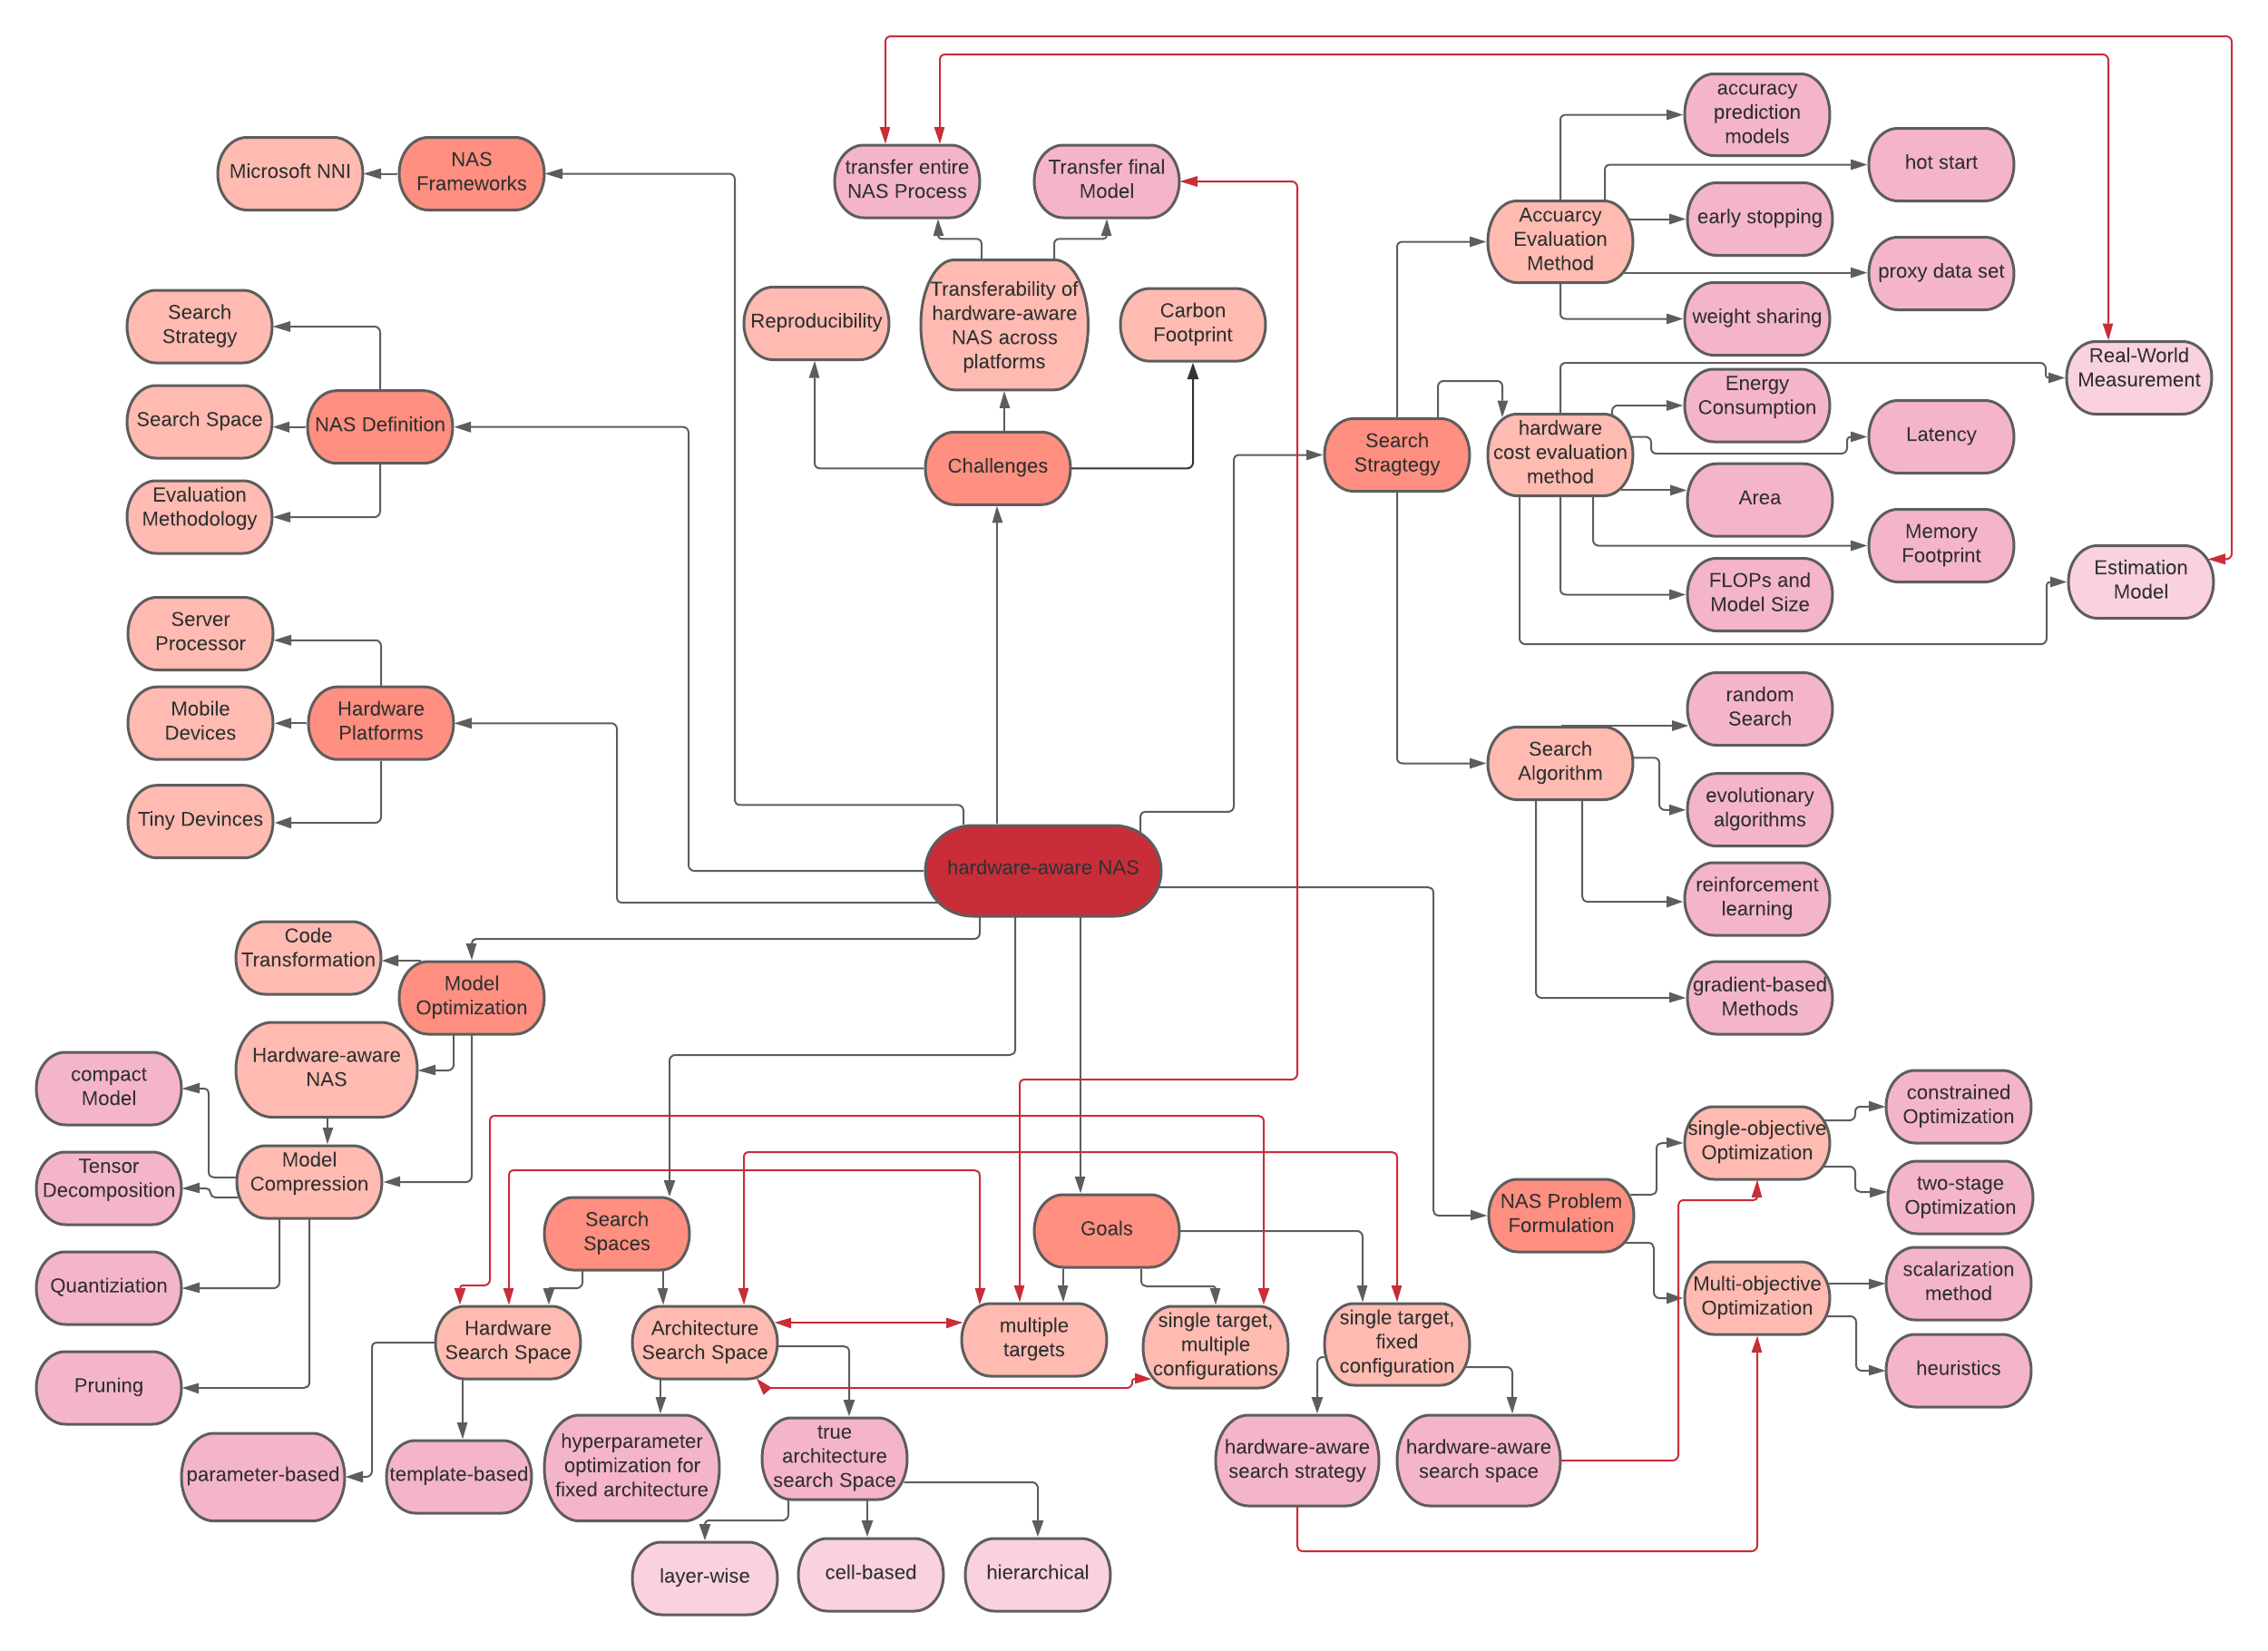
\includegraphics[width=\paperwidth, angle =90]{harware-awareNAS.png}
\caption{Mindmap of paper content}
\label{fig:Mindmap}
\end{figure*} 

\end{document}
